\documentclass[11pt, oneside]{article}   	% use "amsart" instead of "article" for AMSLaTeX format
\usepackage{geometry}                		% See geometry.pdf to learn the layout options. There are lots.
\geometry{letterpaper}                   		% ... or a4paper or a5paper or ... 
%\geometry{landscape}                		% Activate for for rotated page geometry
%\usepackage[parfill]{parskip}    		% Activate to begin paragraphs with an empty line rather than an indent
\usepackage{graphicx}				% Use pdf, png, jpg, or eps� with pdflatex; use eps in DVI mode
								% TeX will automatically convert eps --> pdf in pdflatex		
\usepackage{amssymb}
\usepackage{amsmath}
\usepackage{parskip}
\usepackage{color}
\usepackage{hyperref}

\title{Napkin ring problem}
%\author{The Author}
%\section{}
%\subsection*{}
\date{}							% Activate to display a given date or no date

\graphicspath{{/Users/telliott_admin/Dropbox/Tex/png/}}
% \begin{center} 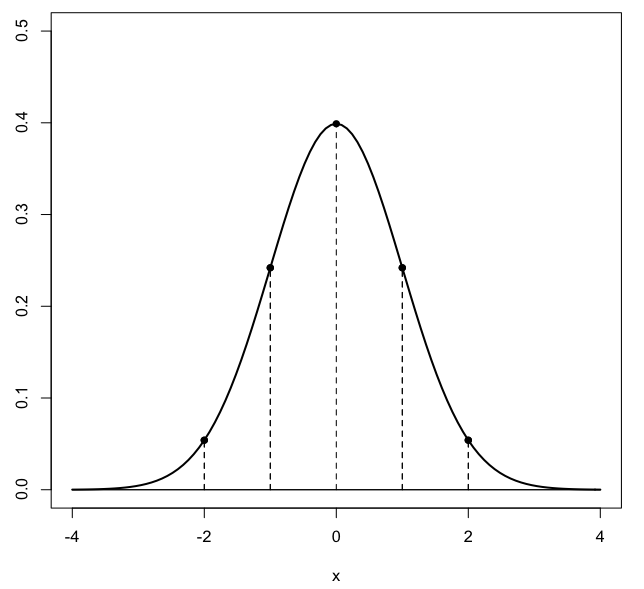
\includegraphics [scale=0.4] {gauss3.png} \end{center}
\begin{document}
\maketitle
\Large
Given a sphere of radius $R$, construct a cylinder of radius $r$ and height $2s$ inside the sphere.

\begin{center} 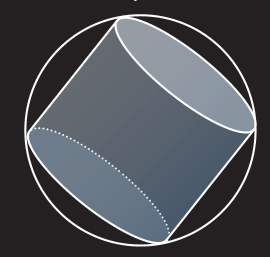
\includegraphics [scale=0.4] {napkin_ring.png} \end{center}

Both the upper and lower edges of the cylinder lie completely on the surface of the sphere.  

To see this, visualize the cross-section through the center of the sphere (and along the axis of the cylinder):  it is just a rectangle inside a circle.

\begin{center} 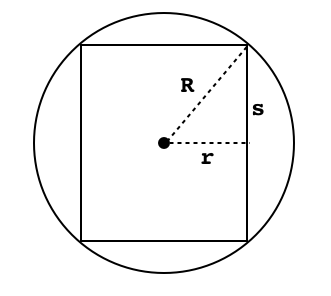
\includegraphics [scale=0.4] {napkin_ring2.png} \end{center}

Rotate this cross section around its vertical axis and obtain our object.  Now we want to treat $r$ as a variable and impose the constraint that the volume of the cylinder is a maximum.  The crucial relationships are that

\[ 0 < r < R \]

because at the extremes the volume of the cylinder will be zero.  And that

\[ r^2 + s^2 = R^2 \]

Compute the two volumes, take their ratio, and maximize that.

\[ V_c = \pi r^2 \cdot 2s \]
\[ V_s = \frac{4}{3} \pi R^3 \]

\[ F = \frac{V_c}{V_s} = \frac{\pi r^2 \cdot 2s }{4/3 \  \pi R^3} = \frac{3}{2} \ \frac{r^2 s}{R^3} \]

From above, we have that

\[ s = \sqrt{R^2 - r^2} \]

So

\[ F = \frac{3}{2} \ \frac{r^2 \sqrt{R^2 - r^2}}{R^3} \]

Set the slope of the derivative equal to zero

\[ \frac{dF}{dr} = 0 = \frac{3}{2R^3} \ \frac{d}{dr} r^2 \sqrt{R^2 - r^2} \]

Since $R \ne 0$, we must have

\[ \frac{d}{dr} r^2 \sqrt{R^2 - r^2} = 0 \]
\[ -2r^3 \ \frac{1}{2} \frac{1}{\sqrt{R^2 - r^2}} + 2r \ \sqrt{R^2 - r^2} = 0 \]
\[ r^2 \ \frac{1}{2} \frac{1}{\sqrt{R^2 - r^2}} = \sqrt{R^2 - r^2} \]
\[ r^2 = 2(R^2 - r^2) \]
\[ 3r^2 = 2R^2 \]
\[ r = \sqrt{\frac{2}{3}} R \]

The answer given here:

url{www.datagenetics.com/blog/july22014/index.html}

is that the ratio of the volumes at the maximum is $1/\sqrt{3}$.

Our expression for the ratio was 

\[ F = \frac{3}{2} \ \frac{r^2 \sqrt{R^2 - r^2}}{R^3} \]

Our answer above:

\[ r = \sqrt{\frac{2}{3}} R \]
\[ r^2 = \frac{2}{3} R^2 \]

So, plugging in:

\[ F = \frac{3}{2} \  \frac{2}{3} R^2 \ \frac{1}{R^3} \ \sqrt{R^2 -  \frac{2}{3} \ R^2}  \]

\[ = \frac{1}{R} \ \sqrt{R^2 -  \frac{2}{3} \ R^2} \]
\[ = \sqrt{\frac{1}{3}} \]



\end{document}  